% Macro Definitions for Operators used in this file
\newcommand{\loft}[5]{\ensuremath{\textcolor{magenta}{\Omega{\bf \mathcal{L}}_{#1}^{#2,#3}}[\textcolor{blue}{\{#4\}}\textcolor{red}{(#5)}]}}

\newcommand{\affine}[5]{\ensuremath{\textcolor{magenta}{\Delta{\bf \mathcal{A}}_{#1}^{#2,#3}} [\textcolor{blue}{\{#4\}} \textcolor{red}{(#5)}]}}

\newcommand{\boolop}[5]{\ensuremath{\textcolor{magenta}{\Omega{\bf \mathcal{B}}_{#1}^{#2,#3}}[\textcolor{blue}{\{#4\}} \textcolor{red}{(#5)}]}}

\newcommand{\generic}[7]{\ensuremath{\textcolor{magenta}{#1{\bf \mathcal{#2}}_{#3}^{#4,#5}}[\textcolor{blue}{\{#6\}} \textcolor{red}{(#7)}]}}


%----------------------------------------------------------------------------------------------------------------------

\begin{frame}{New Form Features Representation}

\begin{itemize}[noitemsep,label=\textbullet,topsep=2pt,parsep=2pt,partopsep=2pt]
\item Snyder \cite{Snyder1992} gave limited set of shapes by {\em Sweep}. 
\item A more generic operation would be {\em Loft}
	\begin{itemize}[noitemsep,label=\textbullet,topsep=2pt,parsep=2pt,partopsep=2pt]
	\item Primitives like {\em Box, Cylinder, Cone, Torus, Sphere} 
	\item Features like {\em Extrude, Revolve, Sweep, Loft}
	\end{itemize}
\item Generic {\em Affine Transformation} operator. 
\item Generic Boolean with a difference of only  'which cells to retain' logic.
\end{itemize}
\begin{center}\includegraphics[width=0.5\linewidth]{../Common/images/SweptVolumes}\end{center}
\end{frame}


%----------------------------------------------------------------------------------------------------------------------

\begin{frame}{ICE scheme \cite{Hoda2005}}

\begin{itemize}[noitemsep,label=\textbullet,topsep=2pt,parsep=2pt,partopsep=2pt]
\item[] Fundamental entities: {\em point} $\bar{p}$ and {\em Regulator}

\vspace{5mm}
{\Large \generic{category}{R}{instance}{subtype}{dimension}{arguments}{shapes}}
\vspace{5mm}

	 For example ,  	\affine{}{T}{1}{\bar{p},line,n}{shape} ,	where,

		\begin{itemize}[noitemsep,label=\textbullet,topsep=2pt,parsep=2pt,partopsep=2pt]
		\item 	\textcolor{magenta}{$\Delta$} : Transformation category (type)
	     	\item 	\textcolor{magenta}{${\bf \mathcal{A}}$} : Affine Transformation regulator (type)
		\item  	\textcolor{magenta}{$^T$}: subtype Translation (type)
		 \item 	\textcolor{magenta}{$^1$} : dimensionality of output (integer)
	        \item 	\textcolor{blue}{ $\bar{p}$} : position (point)
  		\item  	\textcolor{blue}{$line$} : linear guide (curve)
		 \item  	\textcolor{blue}{$n$} : number, used for copies, scaling etc (float)
		 \item  	\textcolor{red}{$shape$} : target (shape)
		\end{itemize}
\end{itemize}
%\includegraphics[scale=0.4]{../Common/images/Letters.png}
\end{frame}


%----------------------------------------------------------------------------------------------------------------------
\begin{frame}{New enhancements to ICE}

\begin{itemize}[noitemsep,label=\textbullet,topsep=2pt,parsep=2pt,partopsep=2pt]
\item{\em Regulator} further classified into 3 components: 
	\begin{itemize}[noitemsep,label=\textbullet,topsep=2pt,parsep=2pt,partopsep=2pt]
	\item \textcolor{magenta}{Operator} : Type-Subtype and dimensionality% of the output.
	\item \textcolor{blue}{Guide-Directrix} : Arguments, Guide-curve
	\item \textcolor{red}{Shape}: Operand
	\end{itemize}
\item {\em point}, {\em line} are present in ICE but not the entities and features pertinent to Mechanical CAD are not. 
\item Our new additions to ICE are:
	\begin{itemize}[noitemsep,label=\textbullet,topsep=2pt,parsep=2pt,partopsep=2pt]
	\item {\bf Entities} : CAD objects like {\em profile}, {\em sketch} etc.
	\item {\bf Regulator}: Changed the definition to include $guide$ (directrix) and removed hard coded $\bar{t}, d$
	\item {\bf Class Hierarchy} : Inheritance {\em child::parent} relationships. %Operations  defined on{\em parent} are applicable to {\em child} classes as well.
	\item {\bf Form Features} : Definitions of variety of {\em form features} and operations like patterning etc.
	\end{itemize}
\end{itemize}
\end{frame}

%----------------------------------------------------------------------------------------------------------------------
\begin{frame}{Entities ($\mathcal{E}$))}
In ICE, fundamental primitive is the {\em point}. %All other geometric  entities are directly or indirectly defined in terms of points. 

\begin{itemize}[noitemsep,label=\textbullet,topsep=2pt,parsep=2pt,partopsep=2pt]%[noitemsep,topsep=2pt,parsep=2pt,partopsep=2pt,label={},leftmargin=*]

\item {\bf Shape} ($shape$): A base class. All other entities directly or indirectly derive from it.

\item {\bf Point} ($point::shape$): A fundamental primitive expressed as $\bar{p}$. 	

\item {\bf Line} ($line::curve$): Defined by two points ($\bar{s_1}$ and $\bar{s_2}$), is expressed as a Loft of $\bar{s_1}$ along {\em line} with $\bar{s_1}$ as start point and $\bar{s_2}$ as end point. \loft{}{T}{1} {0,line ,0} {\bar{s_1} )^{<1>} }	

%\item  {\bf Arc} ($arc::curve$): Defined by three points, embedding angle $\theta$ and is expressed as a Loft of $\bar{s_1}$ along circular path with axis $\bar{t}$ and angle $\theta$. \loft{}{R}{1} {\bar{p},\bar{t}, \theta,n} {\bar{s} )^{<0-1>}}	
%
%\item {\bf Circle} ($circle::curve$) An $arc$ with full rotation, thus having $\theta = 2\pi$ and is expressed as \loft{}{R}{1} {\bar{p},\bar{t}, 2\pi,n} {\bar{s} )^{<0-1>}} 

\item {\bf Curve} ($curve::shape$): A generic entity modeled in terms of $n$ points expressed as \loft{}{C}{1} {0,0,C_{0|1|2}} {\bar{s} )^{<1-n>}} 

%
%\item {\bf Polygon} ($polygon::shape$): Collection of $n$ connected $line$ segments and is expressed as \generic{\Pi}{C}{}{P}{1}{C_0}{line)^{<1-n>}}	

\item {\bf Profile} ($profile::shape$): Collection of $n$ connected $curve$ segments and  is expressed as \generic{\Pi}{C}{}{P}{1}{0,0,C_{0|1|2}}{curve)^{<1-n>}} 

\item {\bf Sketch} ($sketch::shape$): Collection of $profiles$, first outer and rest  inner  and is expressed as \generic{\Pi}{C}{}{S}{1}{}{profile)^{<1><2-n>}}			
%\item {\bf Ruled Surface} ($ruledSurface::shape$): Sweeping of a line along a curve and is expressed as \loft{}{T}{2} {0, curve,0} {line}

%
%\item {\bf Surface} ($surface::shape$): Modeled using collection of $U,V$ curves	and is expressed as \loft{}{F}{2} {0,curve{^{<1-n>} },C_{0|1|2}} {curve{^{<1-m>} }}   

%
%\item {\bf Solid} ($solid::shape$): Modeled using generic surfaces and is expressed as \generic{\Pi}{C}{}{R}{3}{0,0,C_{0|1|2}} {surface{^{<1-n>} }}

\end{itemize}
\end{frame}
%----------------------------------------------------------------------------------------------------------------------
\begin{frame}{Affine Transformation Operators ($\mathcal{A}$)}

{\em Affine Transformations} use matrix multiplications and can be performed on entities of various dimensions, like $point (0)$, $curves(1)$, $surface(2)$ and $solid(3)$. 

\begin{itemize}[noitemsep,label=\textbullet,topsep=2pt,parsep=2pt,partopsep=2pt]
\item {\bf Translation} moves $shape$, along $line$ and is expressed as 	\affine{}{T}{0|1|2|3 }{0,line,0} {shape}
\item{\bf Rotation} rotates $shape$, along $arc$ about point $\bar{p}$ and is expressed as 	\affine{}{R}{0|1|2|3 }{0,arc,0} {shape}	
\item {\bf Scaling} scales $shape$, by factor  $f$, about $axis$ and is expressed as 	\affine{}{S}{0|1|2|3 }{0,axis,f} {shape}	
\end{itemize}

Copy commands like {\em Pattern} can be modeled as {\em Affine Transformations} with $n$ copies.

\begin{itemize}[noitemsep,label=\textbullet,topsep=2pt,parsep=2pt,partopsep=2pt]%[noitemsep,topsep=2pt,parsep=2pt,partopsep=2pt,label={},leftmargin=*]
\item {\bf Linear Pattern} copies $shape$ linearly and is expressed as \affine{}{T}{0|1|2|3 }{0,line,n} {shape} 
\item {\bf Circular Pattern} copies $shape$ circularly and is expressed as \affine{}{R}{0|1|2|3 }{0,arc,n} {shape} 
%\item {\bf Mirror} makes a single copy, mirror-ed about $\bar{t}$ and is expressed as \affine{}{M}{0|1|2|3 }{\bar{p},\bar{t}, 0,1} {shape}	
\end{itemize}

\end{frame}

%----------------------------------------------------------------------------------------------------------------------
\begin{frame}{Boolean Operators ($\mathcal{B}$)}
Boolean operations are also generic in the sense that they can apply on dimensionalities like $curves(1)$, $surface(2)$ and $solid(3)$.  Here, first shape $shape_0$ is regarded as the {\em target body} and the result of the operation is stored in it. Rest of the shapes are termed as {\em tool bodies}.

\begin{itemize}[noitemsep,label=\textbullet,topsep=2pt,parsep=2pt,partopsep=2pt]
\item {\bf Union} combines all the tool shapes ${shape_{1-k}}$ into master shape $shape_0$ and is expressed as	\boolop{}{U}{1|2|3 }{} {shape_{0-k}} 	
\item {\bf Difference} removes combination of all the tool shapes ${shape_{1-k}}$ from master shape $shape_0$ and is expressed as	\boolop{}{D}{1|2|3 }{} {shape_{0-k}}  
\item {\bf Intersection} keeps only common portion of all the shapes ${shape_{0-k}}$ into master shape $shape_0$ and is expressed as	\boolop{}{I}{1|2|3 }{} {shape_{0-k}} 	 
\end{itemize}
\begin{center}\includegraphics[width=0.4\linewidth]{../Common/images/Booleans.jpg}\end{center}
\end{frame}

%----------------------------------------------------------------------------------------------------------------------
\begin{frame}{Loft Operators ($\mathcal{L}$)}
Loft is a generic operator capable of generating most of the basic shapes. It joins {\em profiles} along a guide {\em curve}. 

\centering 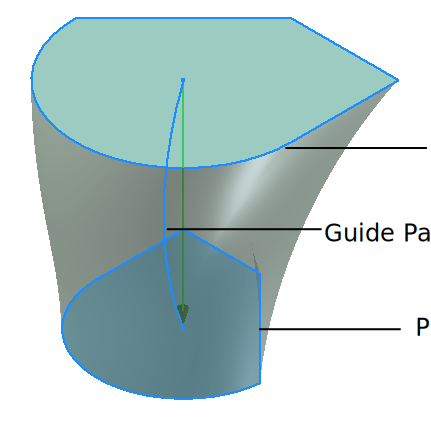
\includegraphics[width=0.8\linewidth]{../Common/images//LoftPreview.pdf} 


Represented as:
\loft{}{subtype}{3}{0, curve, 0 | C_{0,1,2}}{ (sketch )^{<1-n>}}

\end{frame}

%----------------------------------------------------------------------------------------------------------------------
\begin{frame}{Extrude Revolve etc as Loft Operators ($\mathcal{L}$)}

\begin{tabular}{@{}p{0.35\linewidth}p{0.6\linewidth}@{}}

{\bf Loft} can manifest itself in different forms as elaborated below:
{\bf Extrude without draft} is denoted by $EnD$ subtype, has single $sketch$, swept along a $line$ and is expressed as	\loft{}{EnD}{3 }{0,line, 0 | C_0}{ (sketch )^{<1>}}		

Similarly {\em Revolve, Sweep, Loft} (with or without draft) can be expressed as above.

&
\raisebox{-0.9\height}{\includegraphics[width=\linewidth]{../Common/images//LoftExtrudeRevSwp.pdf}}  \\

\end{tabular}

\end{frame}

%----------------------------------------------------------------------------------------------------------------------
\begin{frame}{Primitives as Loft Operators ($\mathcal{L}$)}

\begin{tabular}{@{}p{0.35\linewidth}p{0.6\linewidth}@{}}

By changing shape of the {\em profile} and {\em curve} one can get different standard primitives .

{\bf Box} : {\em Extrude} with {\em Rectangle} as profile shape and is expressed as \loft{}{EnD}{3 }{0,line, 0 | C_0}{ (rectangle )}	

{\bf Cylinder} : {\em Extrude} with {\em Circle} as profile shape and is expressed as \loft{}{EnD}{3 }{0,line, 0 | C_0}{ (circle )}

&
\raisebox{-0.9\height}{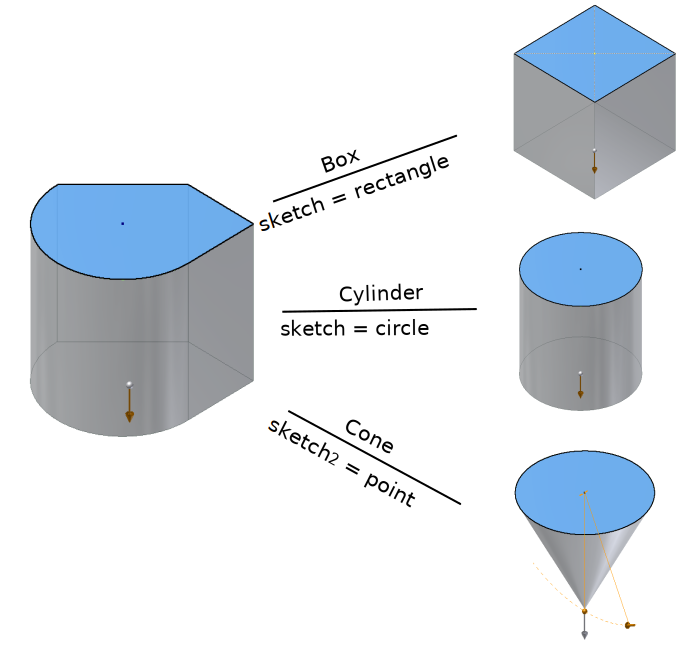
\includegraphics[width=\linewidth]{../Common/images//ExtrudeBoxCylCone.pdf}}  \\

\end{tabular}

\end{frame}

%----------------------------------------------------------------------------------------------------------------------
\begin{frame}{The New Scheme $\mathcal{ABLE}$}
\begin{itemize}[noitemsep,label=\textbullet,topsep=2pt,parsep=2pt,partopsep=2pt]
\item Most of the {\em form features} used in CAD application can be modeled using  three operators, Affine Transformation ($\mathcal{A}$),  Boolean ($\mathcal{B}$) and Loft ($\mathcal{L}$), operating on Entities($\mathcal{E}$). 
\item This representation is called as {\bf $\mathcal{ABLE}$}.  
\item Other features like {\em Shell, Fillet, Chamfer} can also be formulated using {\bf $\mathcal{ABLE}$}. 
\end{itemize}
\end{frame}
%----------------------------------------------------------------------------------------------------------------------
\begin{frame}{Representing Sheet Metal features using  $\mathcal{ABLE}$}
\begin{itemize}[noitemsep,label=\textbullet,topsep=2pt,parsep=2pt,partopsep=2pt]
\item {\bf Face-Wall-Base Flange} can be represented by {\em Extrude} of a given {\em Profile}.
\item {\bf Rib} is a triangular profile extruded.
\item {\bf Hole-Cutout-Slot} is a negative boolean of a tool body which can be represented by  {\em Extrude} of a respective {\em Profile}.
\item {\bf Lance-Louver} is a combination of cutout creation first, then addition of a {\em Sweep} with respective profiles. 
\item {\bf Bend} is a {\em Sweep} of a {\em Rectangular  Profile}	 of edge length. One can add subtype based on the type of relief provided.
\item {\bf Draw-Coin} is a specialized {\em Loft}, with draft, with {\em guide curve} having fillets at the start and end.
\end{itemize}
\begin{center}\includegraphics[width=0.3\linewidth]{../Common/images/SheetMetalFeatures}\end{center}
\end{frame}

%----------------------------------------------------------------------------------------------------------------------
\begin{frame}{Midsurface using $\mathcal{ABLE}$ - Loft}
From {\bf $\mathcal{L}$}, {\em sketches-profiles}, {\em curve} etc are extracted then Midsurface is generated with rules below:
\begin{itemize}[noitemsep,label=\textbullet,topsep=2pt,parsep=2pt,partopsep=2pt]
\item {\bf Thin Sketch}: $sketch_{length} \ll curve_{length}$, then {\em midcurve} is extracted from the {\em sketch} (as mentioned above) and {\em Lofted} with same feature parameters as that of  {\bf $\mathcal{L}$}. 

  \loft{}{L}{2}{0, curve, 0 | C_{0,1,2}}{midcurve^{1-n}} 
\vspace{2mm}
\begin{center}
\includegraphics[width=0.7\linewidth]{../Common/images//MidsurfSmallProfile.pdf}
 \end{center}
\item {\bf Thin Loft} :  $sketch_{length} \gg curve_{length}$, then {\em midcurve} is not extracted  but the {\em sketch} itself is {\em Lofted} along half of the {\em curve}. This rule is expressed as \loft{}{L}{2}{0, curve/2, 0 | C_{0,1,2}}{sketch}.
\end{itemize}
\end{frame}
%----------------------------------------------------------------------------------------------------------------------
\begin{frame}{Midsurface using $\mathcal{ABLE}$ - Booleans}
%For {\bf $\mathcal{B}$} operators rules are devised depending on where the target and tools have Midsurface extracted already.
%\vspace{-0.2cm}

\begin{itemize}[noitemsep,label=\textbullet,topsep=2pt,parsep=2pt,partopsep=2pt]%[noitemsep,topsep=2pt,parsep=2pt,partopsep=2pt,label={},leftmargin=*]

\item {\bf Union} : If the {\em target} and the {\em tool bodies} have midsurfaces, extend the midsurfaces to join at the common intersections.

\includegraphics[scale=0.125]{../Common/images//Midsurf_unite.png} 

\item {\bf Difference-Thin} : If {\em target} is thin then irrespective of {\em tool bodies'} thickness, are subtracted.

\includegraphics[scale=0.125]{../Common/images//Midsurf_diffthin.png}

\item {\bf Difference-Thick} : If {\em target} \& {\em tool bodies} are thick and are in {\em Shell} like situation, {\em midcurves} of combined {\em profiles} are {\em Lofted}  

\includegraphics[scale=0.115]{../Common/images//Midsurf_diffthick.png}
\end{itemize}
\end{frame}

%----------------------------------------------------------------------------------------------------------------------
\begin{frame}{Limitations $\mathcal{ABLE}$}
\begin{itemize}[noitemsep,label=\textbullet,topsep=2pt,parsep=2pt,partopsep=2pt]
\item Not all form features are readily convertible to Sweep/Loft Representations. Complexities arise especially in application specific features like, Louver etc.
\item Tweak features like Fillet and Chamfer are not straight forward, intuitive to represent. Needs a different boolean type.
\item For Free-form Features, sampling of the sections decide fidelity with which its Loft representation can be achieved.
\item Persistent Naming issue, has not yet been considered in this work.
\end{itemize}
\begin{center}\includegraphics[width=0.5\linewidth]{../Common/images/ComplexSweep.jpg}\end{center}
\end{frame}
